\documentclass{article}

\usepackage{amsmath}
\usepackage{booktabs}
\usepackage{fullpage}
\usepackage{parskip}
\usepackage{tikz}
\usetikzlibrary{calc, shapes, patterns}

\begin{document}

\section*{\centering{Moran process}}
\subsection*{\centering{Fitness}}


\[
N=3 
\text{ and } 
A = 
\begin{pmatrix}
    0 & 3 \\ 
    1 & 2
\end{pmatrix}
\]

\vspace{1cm}

\begin{center}
    \begin{tabular}{r|c|c}
        \toprule
                         & \(f(\text{Hawk})\)           & \(f(\text{Dove})\) \\
        \midrule
                         &                              & \\
        1 Hawk, 2 Doves  & \(0\times 0  + 3\times 2\)=6 & \phantom{\(0\times 0 + 3\times 2\)=6} \\
                         &                              & \\
        \midrule
                         &                              & \\
        2 Hawks, 1 Dove  &                              & \\
                         &                              & \\
        \bottomrule
    \end{tabular}
\end{center}

\subsection*{\centering{Probabilities}}

\begin{center}
    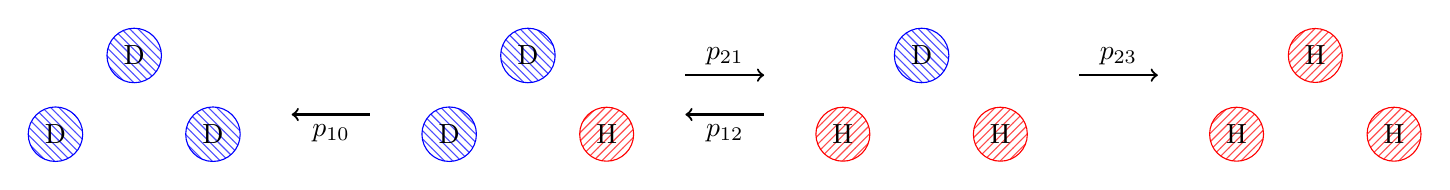
\begin{tikzpicture}[
        dove/.style={circle, pattern=north west lines, pattern color=blue!70, draw=blue},
        hawk/.style={circle, pattern=north east lines, pattern color=red!70, draw=red},
        ]

	\node (N1) at (1, 1) [dove] {D};
	\node (N2) at (0, 0) [dove] {D};
	\node (N3) at (2, 0) [dove] {D};

    \draw [thick, <-] ($(N1)!0.5!(N2) + (2.5, -.25)$) -- node [below] {\(p_{10}\)} ++(1, 0);

    \node (N1) at ($(N1) + (5, 0)$) [dove] {D};
    \node (N2) at ($(N2) + (5, 0)$) [dove] {D};
    \node (N3) at ($(N3) + (5, 0)$) [hawk] {H};

    \draw [thick, <-] ($(N1)!0.5!(N2) + (2.5, -.25)$) -- node [below] {\(p_{12}\)} ++(1, 0);
    \draw [thick, ->] ($(N1)!0.5!(N2) + (2.5, .25)$) -- node [above] {\(p_{21}\)} ++(1, 0);

    \node (N1) at ($(N1) + (5, 0)$) [dove] {D};
    \node (N2) at ($(N2) + (5, 0)$) [hawk] {H};
    \node (N3) at ($(N3) + (5, 0)$) [hawk] {H};

    \draw [thick, ->] ($(N1)!0.5!(N2) + (2.5, .25)$) -- node [above] {\(p_{23}\)} ++(1, 0);

    \node (N1) at ($(N1) + (5, 0)$) [hawk] {H};
    \node (N2) at ($(N2) + (5, 0)$) [hawk] {H};
    \node (N3) at ($(N3) + (5, 0)$) [hawk] {H};
    \end{tikzpicture}
\end{center}

\vspace{1cm}

\begin{center}
    \begin{tabular}{r|c|c}
        \toprule
                     & Selection: Hawk Birth   & Selection: Hawk Death   \\
        \midrule
                     &                                                                          & \\
        \(p_{10}\)   & \(\frac{f(\text{Hawk})}{f(\text{Hawk}) + 2f(\text{Dove})}=\frac{6}{12}\) & \(\frac{1}{3}\)\\
                     &                                                                          & \\
                     &                                                                          & \\
        \(p_{12}\)   &                                                                          & \\
                     &                                                                          & \\
        \midrule
                     &                                                                          & \\
        \(p_{21}\)   &                                                                          & \\
                     &                                                                          & \\
                     &                                                                          & \\
        \(p_{23}\)   &                                                                          & \\
                     &                                                                          & \\
        \bottomrule
    \end{tabular}
\end{center}

\newpage
\section*{\centering{Simulation}}

Use the appropriate dice to simulate 1 Hawk taking over a population of Doves.

Decide what dice you will use to sample birth/death selection at all possible
states:

\begin{center}
    \begin{tabular}{r|c|c|c|c}
        \toprule
        State & Birth: dice used & Select Hawk values   & Death: dice used &
        Select Hawk values \\
        \midrule
                        &   &                 &   & \\
        1 Hawk          & 6 & \(\{1, 2, 3\}\) & 6 & \(\{1, 2\}\) \\
                        &   &                 &   & \\
        \midrule
                        &   &                 &   & \\
        2 Hawks         &   &                 &   & \\
                        &   &                 &   & \\
        \bottomrule
    \end{tabular}
\end{center}


\subsection*{\centering{Example}}

\begin{center}
    \begin{tabular}{r|c|c|c|c|c}
        \toprule
        State & Birth: dice used & Birth: value rolled & Death: dice used & Death: value rolled & Next state   \\
        \midrule
                      &                  &              &                  &              &              \\
        1 Hawk        & 6                &     2        & 6                &             1& 1 Hawk       \\
                      &                  & (Select Hawk)&                  & (Select Hawk)&              \\

                      &                  &              &                  &              &              \\
        1 Hawk        & 6                &     3        & 6                &             5& 2 Hawks      \\
                      &                  & (Select Hawk)&                  & (Select Dove)&              \\
                      &                  &              &                  &              &              \\
        2 Hawks       & 8                &     7        & 6                &             2& 1 Hawk       \\
                      &                  & (Select Dove)&                  & (Select Hawk)&              \\
                      &                  &              &                  &              &              \\
        1 Hawk        & 6                &     4        & 6                & 1& \framebox{0 Hawks}      \\
                      &                  & (Select Dove)&                  & (Select Hawk)&              \\
        \bottomrule
    \end{tabular}
\end{center}

\subsection*{\centering{Activity}}

Every time you arrive at 0 \textbf{or} 3 Hawks: 

\begin{enumerate}
    \item Stop;
    \item Circle your final state
    \item Draw a line in the table (next page);
    \item Start again.
\end{enumerate}

\newpage

\begin{center}
    \begin{tabular}{r|c|c|c|c|c}
        \toprule
        Current state & Birth: dice used & Birth: value rolled & Death: dice used & Death: value rolled & Next state   \\
        \midrule
        1 Hawk        & 6                &              &                  &              &              \\
                      &                  &              &                  &              &              \\
                      &                  &              &                  &              &              \\
                      &                  &              &                  &              &              \\
                      &                  &              &                  &              &              \\
                      &                  &              &                  &              &              \\
                      &                  &              &                  &              &              \\
                      &                  &              &                  &              &              \\
                      &                  &              &                  &              &              \\
                      &                  &              &                  &              &              \\
                      &                  &              &                  &              &              \\
                      &                  &              &                  &              &              \\
                      &                  &              &                  &              &              \\
                      &                  &              &                  &              &              \\
                      &                  &              &                  &              &              \\
                      &                  &              &                  &              &              \\
                      &                  &              &                  &              &              \\
                      &                  &              &                  &              &              \\
                      &                  &              &                  &              &              \\
                      &                  &              &                  &              &              \\
                      &                  &              &                  &              &              \\
                      &                  &              &                  &              &              \\
                      &                  &              &                  &              &              \\
                      &                  &              &                  &              &              \\
                      &                  &              &                  &              &              \\
                      &                  &              &                  &              &              \\
                      &                  &              &                  &              &              \\
                      &                  &              &                  &              &              \\
                      &                  &              &                  &              &              \\
                      &                  &              &                  &              &              \\
                      &                  &              &                  &              &              \\
                      &                  &              &                  &              &              \\
                      &                  &              &                  &              &              \\
                      &                  &              &                  &              &              \\
                      &                  &              &                  &              &              \\
                      &                  &              &                  &              &              \\
                      &                  &              &                  &              &              \\
                      &                  &              &                  &              &              \\
                      &                  &              &                  &              &              \\
                      &                  &              &                  &              &              \\
                      &                  &              &                  &              &              \\
                      &                  &              &                  &              &              \\
                      &                  &              &                  &              &              \\
                      &                  &              &                  &              &              \\
                      &                  &              &                  &              &              \\
                      &                  &              &                  &              &              \\
                      &                  &              &                  &              &              \\
    \end{tabular}
\end{center}

\end{document}

